%!TEX root = draft.tex
%\newcommand{\seqPQ}{\mathsf{SeqPQ}}

\section{Compositionality of Distributed Linearizability}
\label{sec:compositionality of distributed linearizability}

%We assume that given a multi-object history $h$, According to causal-delivery of CRDT, in this section, given a multi-object history $h$, we assume that for each object $\mathit{obj}$, the visibility relation of

The following is the definition of distributed linearizability for multi-object histories.

\begin{definition}[Distributed Linearizability for Multi-object Histories]
\label{definition:distributed linearizability for multi-object histories}
A history $h$ of multiple objects is distributed linearizabile, if there exists a sequence $\mathit{lin}$, called linearization of $h$, such that

\begin{enumerate}[(i)]
\item The elements of $\mathit{lin}$ is generated from the operations of $h$: each operation $o = (m(a) \Rightarrow b,i,\mathit{obj})$ is transformed into $(m(a) \Rightarrow b,i,S)$ with $S$ set of identifiers of operations of visible to $o$ via $h.\mathit{vis}$.
\item $\mathit{lin}$ is consistent with $h. \mathit{vis}$.
\item For each object $\mathit{obj}$, $h \uparrow_{\mathit{obj}}$ is distributed linearizable, and $\mathit{lin} \uparrow_{ \mathit{obj} }$ is a linearization of $h \uparrow_{\mathit{obj}}$.
\end{enumerate}

A set $H$ of multi-object histories are distributed linearizable w.r.t deterministic sequential specifications, if each of its history is.
\end{definition}

The following is the definition of compositional histories.

\begin{definition}[Compositionality]
\label{definition:compositionality}
A history $h$ of multiple objects is called compositional, if $h \uparrow_{\mathit{obj}}$ is distributed linearizable for each object $\mathit{obj}$, if and only if, $h$ is distributed linearizable.
\end{definition}

It is easy to see that, a multi-object history $h$ being distributed linearizable implies that the projection of $h$ into each object is distributed linearizable. When proving compositionality, we only need to consider the opposite direction.




\subsection{Composing Several t0-Specifications}
\label{lemma:several t0-specifications can be composed}

The following lemma states that a history of several objects of t0 specifications is compositional. Its proof can be found in Appendix \ref{subsec:appendix proofs of lemma several t0-specifications can be composed}.

\begin{restatable}{lemma}{composingTZero}
\label{lemma:several t0-specifications can be composed}
Given a multi-object history $h$, if each of its object uses a t0-specification, then, $h$ is compositional.
\end{restatable} 




\subsection{Composing Several t0-Specifications with One T1-specification}
\label{lemma:composing several t0-specification with one t1-specification}

Composing several t0-specifications with one t1-specification does not hold in general. \figurename~\ref{fig:a failed example of composing a multi-value register with a last-write-win register} is a history $h$ that is a failed example of composing a multi-value register with a last-write-win register, where the operations of LWW register are boxed. Here we assume that $\mathit{ts}_1<\mathit{ts}_2$. Since multi-value register is t0-specification and LWW register is t1-specification, we can see that the projection of $h$ into operations of multi-value register is distributed linearization and the only possible linearization is $\mathit{write}(a) \cdot \mathit{write}(b)$, and the projection of $h$ into operations of LWW register is distributed linearization and the only possible linearization is $\mathit{write}(c) \cdot \mathit{write}(d)$. However, $h$ is not distributed linearizable, since there is a a cycle.

\begin{figure}[t]
  \centering
  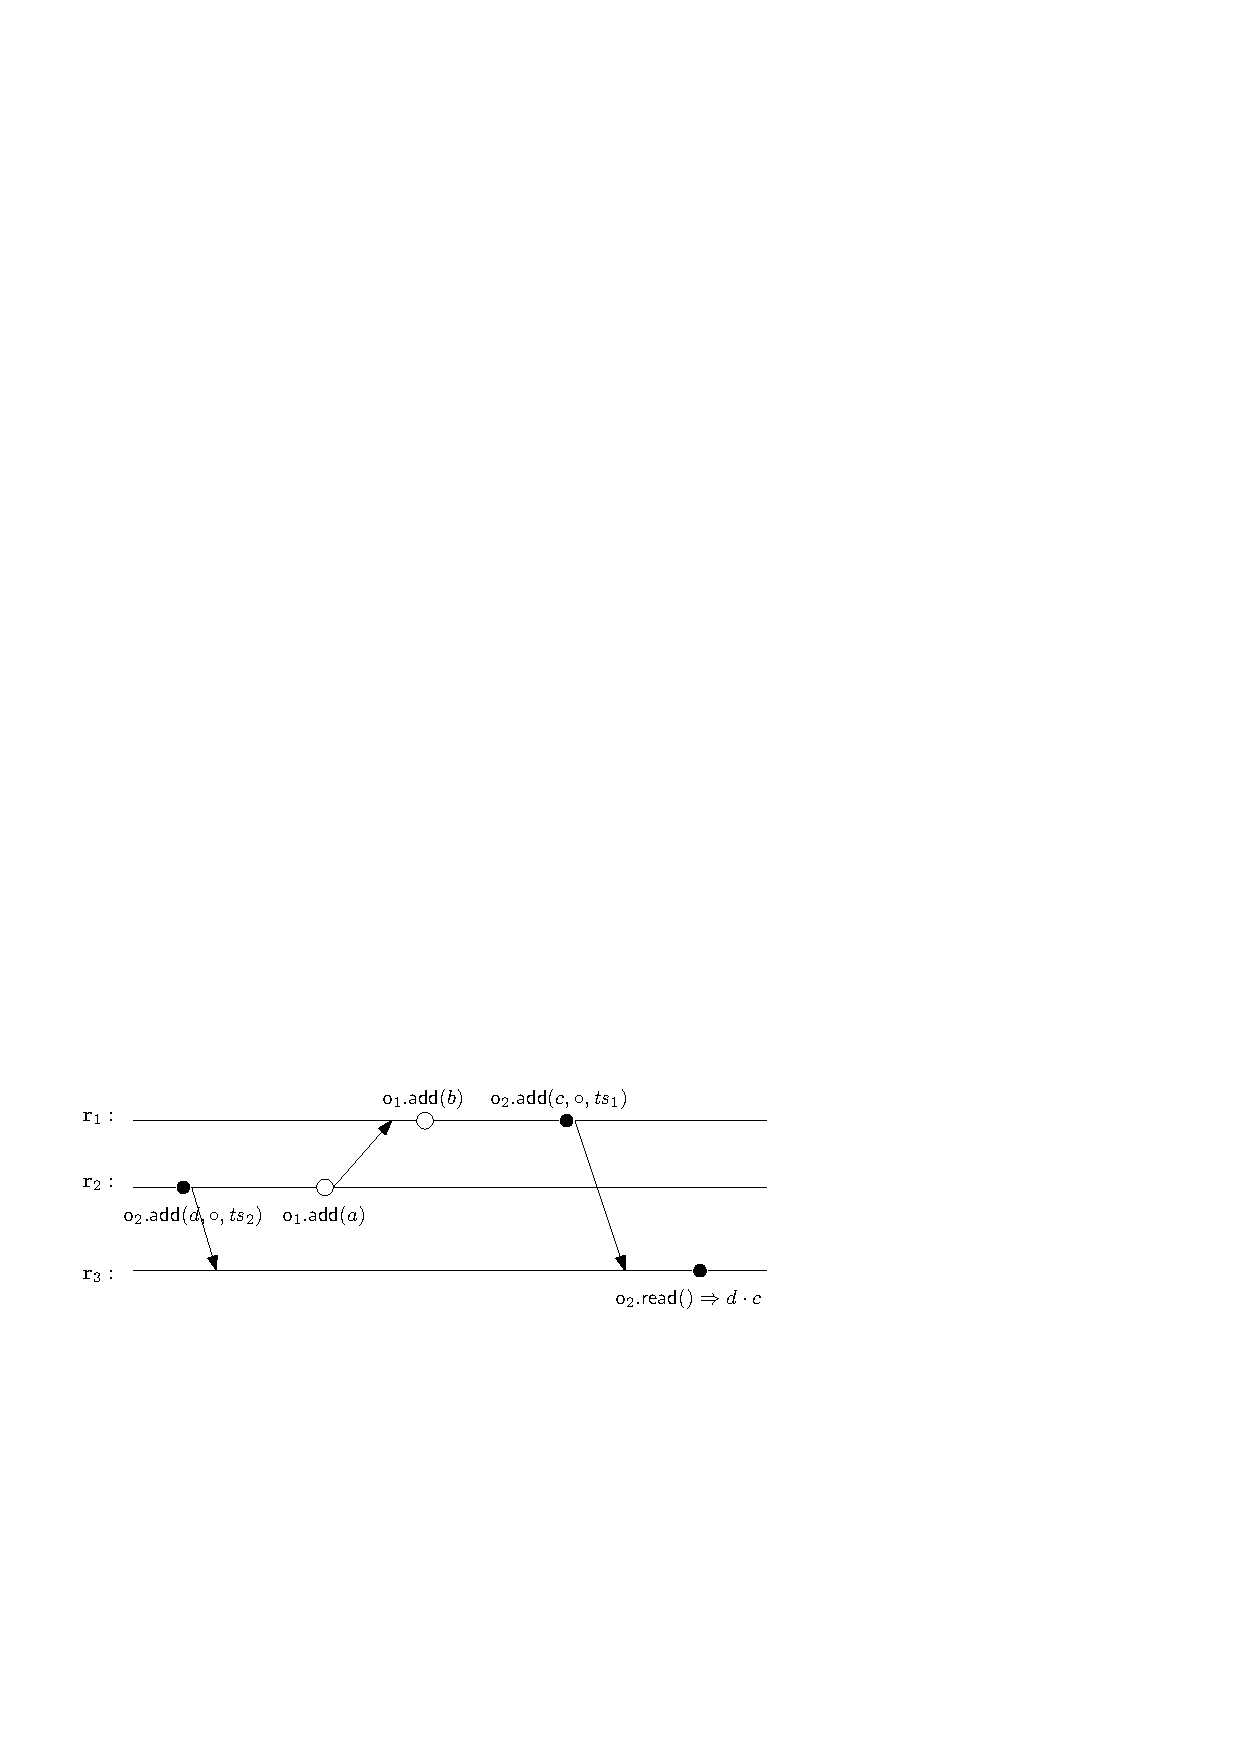
\includegraphics[width=0.6 \textwidth]{figures/MVReg-LWWReg-Nocd.pdf}
\vspace{-10pt}
  \caption{A failed example of composing a multi-value register with a last-write-win register (boxed operations), where $\mathit{ts}_1 < \mathit{ts}_2$.}
  \label{fig:a failed example of composing a multi-value register with a last-write-win register}
\end{figure}

The following lemma states that for a multi-object history, if its object use several t0-specifications and one t1-specification, and its visibility relation is transitive, then, $h$ is compositional. Its proof can be found in Appendix \ref{subsec:appendix proofs of lemma several t0-specifications and one t1-specification can be composed}.

\begin{restatable}{lemma}{composingTZeroAndOneTOne}
\label{lemma:several t0-specifications and one t1-specification can be composed}
Given a multi-object $h$, if its object use several t0-specifications and one t1-specification, and its visibility relation is transitive, then, $h$ is compositional.
\end{restatable} 




\subsection{Composing Several t0-Specifications with Several T1-specification}
\label{lemma:composing several t0-specification with several t1-specification}

Composing several t0-specifications with several t1-specification does not hold in general. \figurename~\ref{fig:a failed example of composing two last-write-win registers} is a history $h$ that is a failed example of composing two last-write-win registers, where the operations of one LWW register are boxed, and the operations of the other LWW registers are not boxed. Here we assume that $\mathit{ts}_1 < \mathit{ts}_2 < \mathit{ts}_3$, and $\mathit{ts}'_1 < \mathit{ts}'_2$. Since LWW register is t1-specification, we can see that the projection of $h$ into operations of one LWW register is distributed linearization and the only possible linearization is $\mathit{write}(a,\mathit{ts}'_1) \cdot \mathit{write}(b,\mathit{ts}'_2)$, and the projection of $h$ into operations of the other LWW register is distributed linearization and the only possible linearization is $\mathit{write}(c,\mathit{ts}_1) \cdot \mathit{write}(d,\mathit{ts}_2) \cdot \mathit{write}(e,\mathit{ts}_3)$. However, $h$ is not distributed linearizable, since there is a a cycle.

\begin{figure}[t]
  \centering
  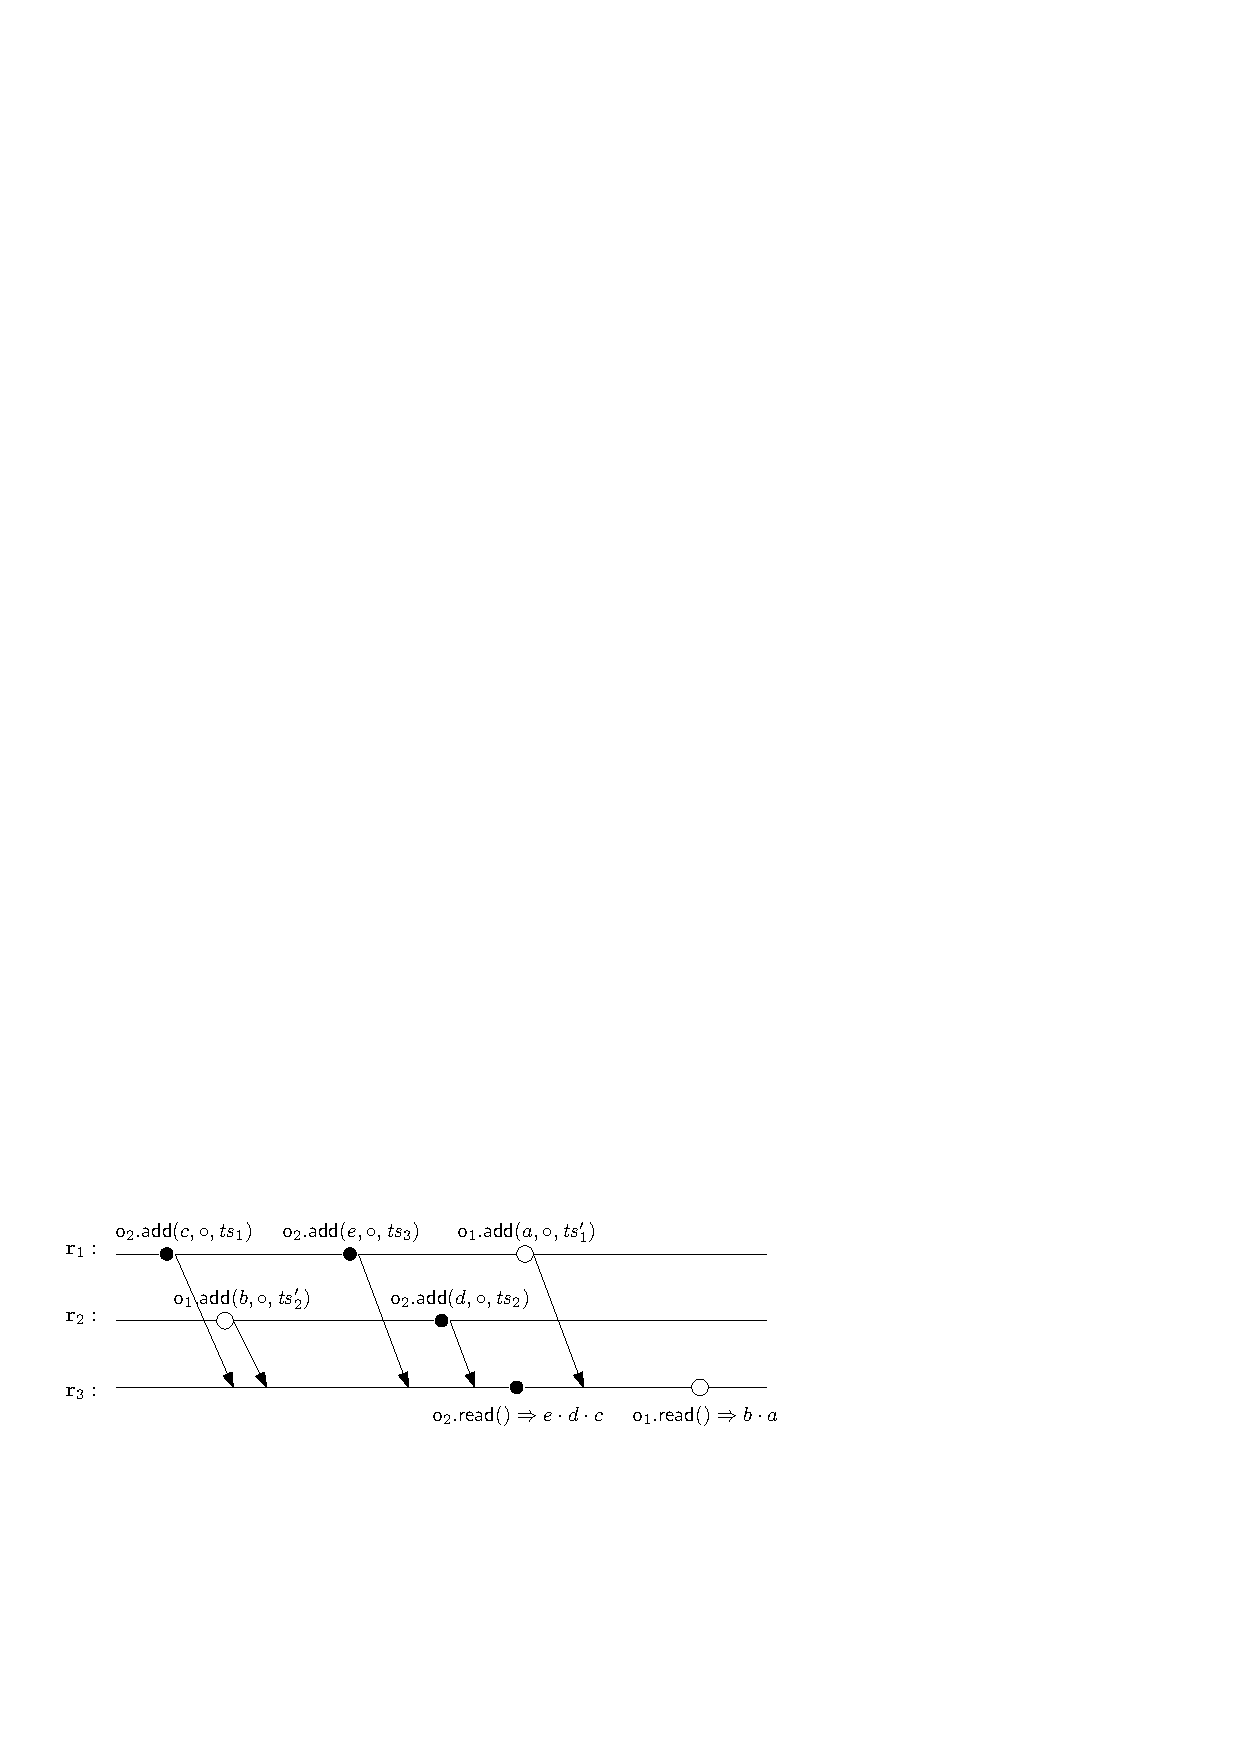
\includegraphics[width=0.7 \textwidth]{figures/LWWReg-LWWReg-NoSTS.pdf}
\vspace{-10pt}
  \caption{A failed example of composing two last-write-win registers (one object is boxed, the other is not), where $\mathit{ts}_1 < \mathit{ts}_2 < \mathit{ts}_3$, and $\mathit{ts}'_1 < \mathit{ts}'_2$.}
  \label{fig:a failed example of composing two last-write-win registers}
\end{figure}


A history $h$ satisfies causal-time-stamp, if: Given operation $o_1,\ldots,o_{\mathit{2k+2}}$ of $h$ that are of objects of t1-specification, if 

\begin{itemize}
\setlength{\itemsep}{0.5pt}
\item[-] $(o_2,o_3)$ are of a same object, $\ldots$, $(o_{\mathit{2k}},o_{\mathit{2k+1}})$ are of a same object, $(o_{\mathit{2k+2}},o_1)$ are of a same object, 

\item[-] $\mathit{ts}(o_2) < \mathit{ts}(o_2)$, $\ldots$, and $\mathit{ts}(o_{\mathit{2k}}) < \mathit{ts}(o_{\mathit{2k+1}})$, 

\item[-] $(o_1,o_2), \ldots, (o_{\mathit{ek+1}},o_{\mathit{2k+2}}) \in \mathit{vis}$. 
\end{itemize} 

Then, we have $\mathit{ts}(o_1) < \mathit{ts}(o_{\mathit{2k+1}})$. 

The following lemma states that for a multi-object history, if its object use several t0-specifications and several t1-specification, and it satisfies causal-time-stamp and its visibility relation is transitive, then, $h$ is compositional. Its proof can be found in Appendix \ref{subsec:appendix proofs of lemma several t0-specifications and several t1-specification can be composed}.

\begin{restatable}{lemma}{composingTZeroAndTOne}
\label{lemma:several t0-specifications and several t1-specification can be composed}
Given a multi-object $h$, if its object use several t0-specifications and several t1-specification, and it satisfies causal-time-stamp and its visibility relation is transitive, then, $h$ is compositional. 
\end{restatable} 



%%% Local Variables:
%%% mode: latex
%%% TeX-master: "draft"
%%% End:
